\section{Fundamentals of Sound}
\begin{frame}{}
    \LARGE \textbf{Fundamentals of Sound}
\end{frame}

\begin{frame}{What is Sound?}
    \begin{figure}
        \centering
        \fetchconvertimage{https://letstalkscience.ca/sites/default/files/styles/x_large/public/2020-01/Sound_waves_and_particles.png}{images/audio-nlp/sound-waves.png}{width=\textwidth,height=0.6\textheight,keepaspectratio}
    \end{figure}
    \begin{itemize}
        % \setlength{\itemsep}{1.5em}
        \item Sound is a type of energy produced by vibrating objects.
        \item It travels through air (or other media) as waves.
        \item Sound waves are longitudinal waves, meaning the particle displacement is parallel to the direction of wave propagation.
    \end{itemize}
\end{frame}

\begin{frame}[allowframebreaks]{Fundamentals of Sound: Physics Concepts}
    \begin{figure}
        \centering
        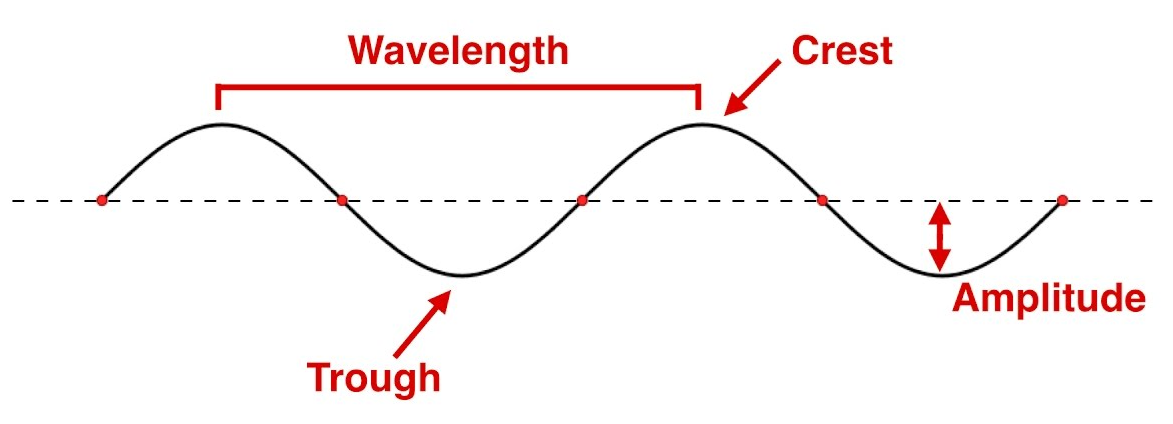
\includegraphics[width=0.8\textwidth]{images/audio-nlp/sound-props.png}
    \end{figure}
    \begin{itemize}
        \item \textbf{Waveform}: The shape of the sound wave, representing how air pressure changes over time.
        \item \textbf{Frequency}: Number of cycles (oscillations) per second, measured in Hertz (Hz). Determines the pitch of the sound.
        \item \textbf{Amplitude}: The height of the wave, representing the loudness or intensity of the sound.
    \end{itemize}
\framebreak
    \begin{itemize}
        \item \textbf{Sampling Theorem (Nyquist)}: To accurately digitize a sound, the sampling rate ($f_s$) must be greater than twice the highest frequency present in the signal ($f_{max}$):
        \[
            f_s > 2f_{max}
        \]
        \item \textbf{Aliasing}: If the sampling rate is too low, higher frequencies are misrepresented as lower frequencies, causing distortion. 
        \begin{center}
            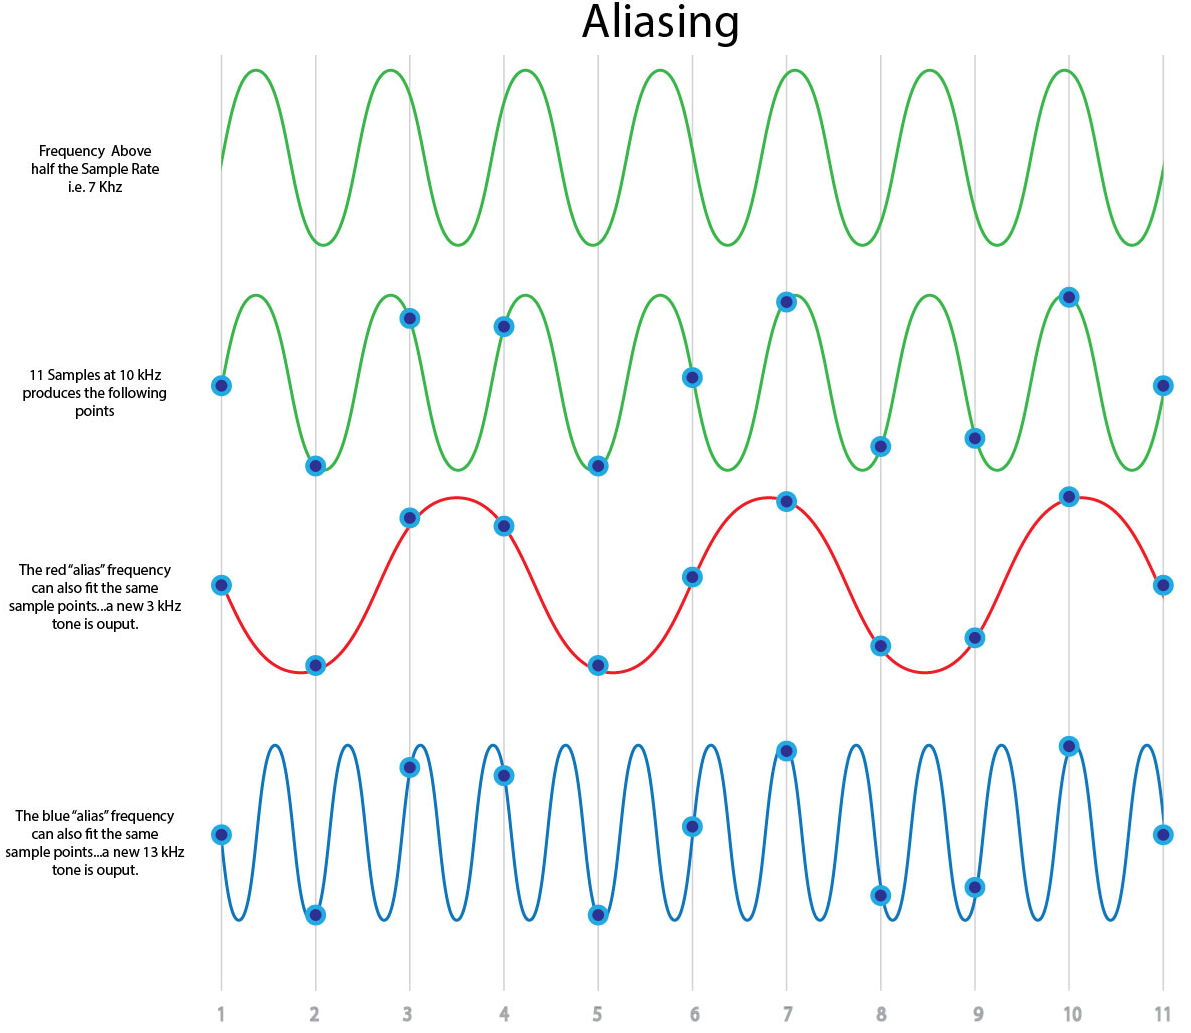
\includegraphics[width=\textwidth,height=0.9\textheight,keepaspectratio]{images/audio-nlp/aliasing.png}
        \end{center}
    \end{itemize}
\end{frame}